\documentclass[a4paper,11pt]{article}
\usepackage[utf8]{inputenc}
\usepackage[french]{babel}
\usepackage{amsmath}
\usepackage[osf,sups]{Baskervaldx} % lining figures
\usepackage[bigdelims,cmintegrals,vvarbb,baskervaldx]{newtxmath} % math font
\usepackage{graphicx}
\usepackage{url,hyperref}

% margins
\setlength{\parindent}{0em}
\setlength{\parskip}{1em}
\addtolength{\hoffset}{-3.5em}
\addtolength{\textwidth}{7em}
\addtolength{\voffset}{-5em}
\addtolength{\textheight}{10em}


\begin{document}
\thispagestyle{empty}

{\bf
	Localisation de modes normaux~:
	application aux galeries de chuchotements
}

{\bf Encadrants}:\\
Rafael Grompone von Gioi \verb+<rafael.grompone@ens-paris-saclay.fr>+\\
Enric Meinhardt-Llopis \verb+<enric.meinhardt@ens-paris-saclay.fr>+ 

{\bf Contexte}\\
Les modes normaux d'une variété compacte~$\Omega$ sont les fonctions propres de
son opérateur de Laplace-Beltrami~$\Delta_\Omega$.  Elles sont typiquement des
fonctions ``globales'', supportées par~$\Omega$ entier.  Le cas d'école est la
corde vibrante~$\Omega=[0,L]$ aux extréma fixés, où les
fonctions propres sont~$\varphi_n(x)=\sin\frac{\pi n x}L$
pour~$n=1,2,3,\ldots$ qui correspondent à des vibrations
de fréquence~$\mu_n=\frac{\pi n}L$ de la corde toute entière.  Sur d'autres
domaines~$\Omega$ la situation est plus intéressante: on voit apparaître
parfois des \emph{modes normaux localisés} sur une toute petite partie
d'$\Omega$.
Ces modes localisés sont le fondement mathématique des ``galeries de
chuchotements'' (\emph{whispering galleries}), des structures architectoniques
où l'on peut parler très bas d'un bout à l'autre de la chambre sans que
personne d'autre puisse entendre la conversation.  Si~$\Omega$ est l'intérieur
de la chambre, il y a des fonctions propres de~$\Delta_\Omega$ qui sont
localisées autour de deux points concrets d'$\Omega$ entre lesquels on peut se
chuchoter.


{\bf Objectif du stage}\\
L'objectif de cet stage est trouver des formes~$\Omega$ pour lesquelles il y a
des modes normaux localisés autour de deux points.
Le problème direct, bien connu, consiste à trouver
les premières fonctions propres du Laplacien sur un maillage décrivant la forme
de l'objet.  En pratique, c'est le calcul du
spectre~$\mathrm{sp}_{\mathbf{R}}(A)$ d'une matrice~$A$ symétrique définie
positive.
On s'intéresse au problème inverse: étant donné un maillage, comment faire
varier la longueur des liens du maillage---la forme de l'objet---de façon que
son spectre coïncide avec un spectre objectif souhaité?
Matriciellement, on se donne un spectre
objectif~$\Sigma\in\mathbf{R}^n$ et une structure de maillage décrite par une
matrice~$B\in\mathrm{M}_{m,n}(\mathbf{R})$, et on doit trouver des
``poids''~$W\in\mathbf{R}^m$ tels
que~$\mathrm{sp}_\mathbf{R}\left(B^T\mathrm{diag}(W)B\right)=\Sigma$.

\setlength{\tabcolsep}{0pt}
\begin{tabular}{ccccccccccc}
	
\includegraphics[width=0.093\linewidth]{f/marsmooth.png} &
	
\includegraphics[width=0.093\linewidth]{f/marbords.png} &
	
\includegraphics[width=0.093\linewidth]{f/marimba_v01.png} &
	
\includegraphics[width=0.093\linewidth]{f/marimba_v02.png} &
	
\includegraphics[width=0.093\linewidth]{f/marimba_v03.png} &
	
\includegraphics[width=0.093\linewidth]{f/marimba_v04.png} &
	
\includegraphics[width=0.093\linewidth]{f/marimba_v05.png} &
	
\includegraphics[width=0.093\linewidth]{f/marimba_v06.png} &
	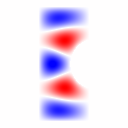
\includegraphics[width=0.093\linewidth]{f/marimba_v07.png} &
	
\includegraphics[width=0.093\linewidth]{f/marimba_v08.png} &
	
\includegraphics[width=0.093\linewidth]{f/marimba_v09.png} \\
	$1\!\!1_\Omega$  & $W$ &
	$\lambda_1$ &
	$\lambda_2$ &
	$\lambda_3$ &
	$\lambda_4$ &
	$\lambda_5$ &
	$\lambda_6$ &
	$\lambda_7$ &
	$\lambda_8$ &
	$\lambda_9$
\end{tabular}

On va résoudre ce problème par force brute, en minimisant
fonction~$W\mapsto\left\|\mathrm{sp}_\mathbf{R}\left(B^TWB\right)-\Sigma\right\|^2$
avec des méthode d'optimisation modernes; notamment celles utilisées
en~\emph{deep-learning}, pour lesquelles ce problème est d'une taille
considérée petite.  Pour cela, il faut une implémentation de la
fonction~$A\mapsto\mathrm{sp}_\mathbf R(A)$ que l'optimiseur puisse dériver
localement.  C'est ici qu'il y aura la plupart du travail du stage, qui
pourrait parfaitement être titré~\emph{``a differentiable implementaion of the
eigenvalues computation''}.

Si le stage amène à une conclusion positive, on pourra soumettre une
publication (première!) sur l'application des méthodes de deep learning à la
modélisation d'instruments musicaux.


\vspace{-1.5em}
\renewcommand{\refname}{\normalsize Références}
%
\begin{thebibliography}{99}
\vspace{-1em}
{\scriptsize
\bibitem{drum}
	Kac, M..
	{\it Can one hear the shape of a drum?}
	The american mathematical monthly, (1966)

\bibitem{inverse}
	Chu, M., \& Golub, G.
	{\it Inverse eigenvalue problems: theory, algorithms, and
	applications}, OUP (2005)

\bibitem{localfun}
	Nguyen, B. \& Grebenkov, D.~S.
	{\it Localization of Laplacian eigenfunctions in circular, spherical
	and elliptical domains}, SIAM J.  Appl. Math. (2019)

\bibitem{geofun}
	Grebenkov, D.~S.  \& Nguyen, B.
	{\it Geometrical structure of Laplacian eigenfunctions},
	SIAM Rev. (2013)

\bibitem{backeigen}
	Wang,~W., Dang,~Z., Hu,~Y., Fua,~P., Salzmann,~M.
	{\it Backpropagation-Friendly Eigendecomposition},
	NeurIPS (2019)

}
\end{thebibliography}



\end{document}  


% vim:set tw=79 spell spelllang=fr:
